\documentclass[11pt,twoside,a4paper]{report}
\usepackage[utf8]{inputenc}
\usepackage{amsmath}
\usepackage{amsfonts}
\usepackage{amssymb}
\usepackage{url}
\usepackage{graphicx}
\usepackage{caption}
\usepackage{subcaption}
\begin{document}

\title{Evaluation of algorithms for complex shielding in point kernel dose calculations}
\author{Tom Robert Bryntesen}
\date{May 2015}
\maketitle

\begin{abstract}
This thesis compares algorithms for finding the intersections with complex shields as part of the point-kernel algorithm. The calculations is used to visualise radiation in real time which require a large number of measurements to be calculated. The shielding calculations is the most time consuming part of the calculation when there is a complex environment. Three algorithms for calculating shielding have been implemented. One uses boolean operations on primitive shapes like boxes, cylinders and spheres to create complex objects. The second uses a triangulated geometry. The third uses a 3D voxel grid. Each algorithm have been benchmarked for performance, accuracy and memory usage. The boolean method is the fastest. For the two others there are a tradeoff between accuracy and performance. However both have similar performance when setup to give the same accuracy.
\end{abstract}

\tableofcontents

\chapter{Introduction}
In the nuclear field the workers are exposed to the risk of being exposed to radiation. In radiation protected the ALARA principle states that the risk shall be as low as reasonably achievable. 

One way to lower the risk is to teach the workers about radiation. Software that visualise the radiation is helpful in that it lets the user see the radiation. Doing so can help teach about the factors in dose uptake. That is time of exposure, distance and shielding. When preparing for a job the worker can be briefed about the procedure by showing an animation with radiation visualisation. It is also possible to train on the procedure actively, in an interactive virtual reality environment. By seeing the risky areas the worker can take steps to avoid the high radiation areas, or minimise the time spent there to get a lower dose. 

Another way to lower the risk is for better planning. Given a planning software that could estimate the doses of workers one could experiment to find the scenario that gives the lowest dose. Either by changing where the workers stand or putting up shielding.

\section{Motivation}
In order to visualise radiation or calculate doses one need to do a great number of calculations. Many visualisation takes a 3 dimensional grid of values as input. If there are 20 cells in each dimension it would require 8000 measurements to generate the visualisation. If the scene is changing, for example when a shield or source is moving, the visualisation has to be updated at interactive rates. 

To calculate the dose of a worker over time one needs to integrate the dose-rate over time. For example the software would calculate the dose-rate for the worker every second and add it all up to get the dose. Thousands of calculations would need to be performed for each worker, if the procedure last more than an hour. So to keep the software responsive the calculation need to be as fast as possible.

There are different ways to represent a radiological scene. If there are measurements in the area then interpolation can be used to estimate the value at an arbitrary position. However this would not allow for a dynamic scene where one can move sources or shields around. Another way is to define sources and shields and calculate the dose-rates from that. Monte carlo methods simulate photons radiating from the source threw the environment until it reaches the measuring position. This is accurate but very slow. The point-kernel method calculates the dose-rate by taking a single ray from the source to the measuring position and uses formulas and statistical data to estimate the dose-rate. This is not as accurate as monte carlo but is very fast. A more indepth description of the calculation methods is given in chapter 2.

One of the inputs to the point-kernel calculation is the how the ray intersects with the shields between the source and measuring position. This is the most time consuming part of the algorithm for a scene with many shields. By improving the performance of the shields calculation the software will run faster giving a better user experience.

This thesis is written in collaboration with Institute for Energy Technology (IFE). They have implemented a point-kernel calculator that is used in their software. It has support for simple shields like boxes and cylinders. They also support a complex shield that uses a triangulated mesh to represent arbitrary shapes. The evaluation of other ways to represent and calculate complex shield can help IFE improve their calculator.

\section{Research Objectives}
The work in this thesis will find alternative ways to represent complex shields. That is shapes that can be arbitrary and concave. Some of the alternatives will be selected and implemented. The implementations will be evaluated and compared. The following research questions will be focused on during the evaluation process:

How fast is the method
How does the shape influence the speed
How accurate is the method
Are the tradeoffs in the way the method are configured, for example between speed, memory and accuracy
How practical is the method
What is the overhead, how suitable is the method for representing simple shapes

Speed, memory and accuracy will be measured using quantitative measures from benchmarks. 

\section{Outline}
Background
Chapter 2 gives an introduction to ionising radiation and methods of calculating doses. How the shield intersections are part of the calculation is explained.  A review of relevant ray tracing algorithms are presented. 
Design
Chapter 3 gives a detailed explanation the design of the shield intersection algorithms and the benchmarking framework. 
Implementation
Chapter 4 gives a detailed description of the implementation of the design described in chapter 3.
Performance Investigation
Chapter 5 shows the results of the benchmarks.
Discussion
Chapter 6 presents the findings from the tests.
Conclusion and Future Research
Chapter 7 gives guidelines on when to use each algorithm, based on the findings from the test. Finally some recommendations for future work are offered.


\chapter{Background}
\section{Radiation Theory}
\section{Monte Carlo}
\section{Point-kernel}
\section{Raytracing}

\chapter{Method}
\section{Benchmarking}
\section{Datasets}
\section{Data Collection}
\section{Data analysis}

\chapter{Design and Implementation}

\begin{figure}[h]
        \centering
        \begin{subfigure}[h]{0.3\textwidth}
                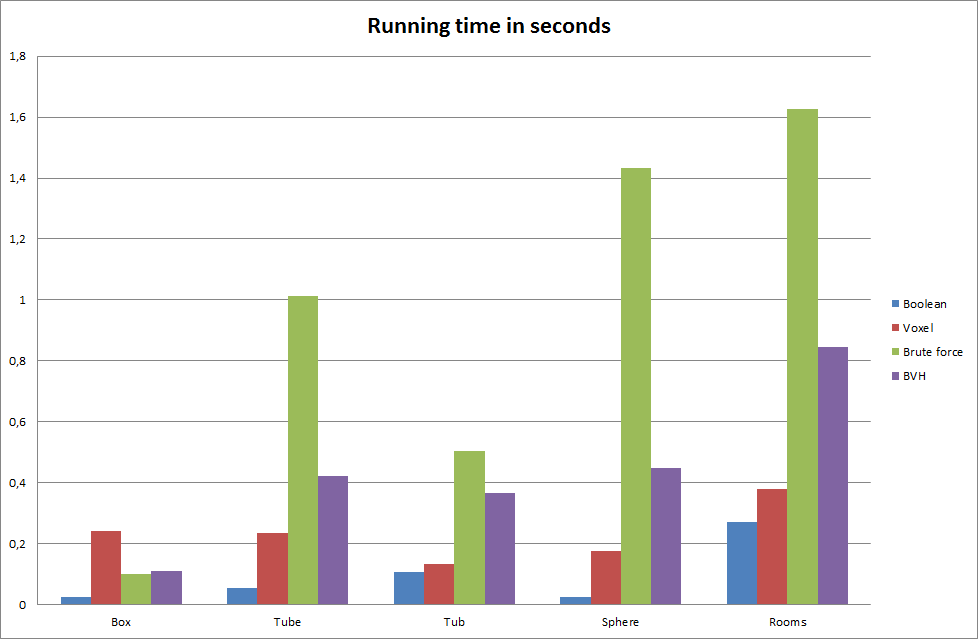
\includegraphics[width=\textwidth]{images/running_time_seconds}
                \caption{A gull}
                \label{fig:gull}
        \end{subfigure}%
        ~ %add desired spacing between images, e. g. ~, \quad, \qquad, \hfill etc.
          %(or a blank line to force the subfigure onto a new line)
        \begin{subfigure}[h]{0.3\textwidth}
                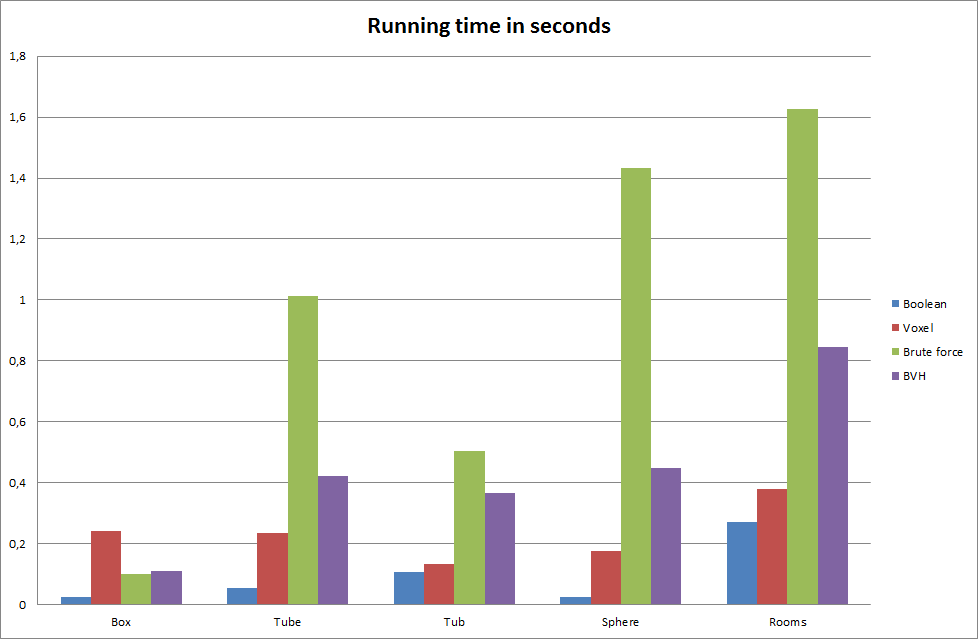
\includegraphics[width=\textwidth]{images/running_time_seconds}
                \caption{A tiger}
                \label{fig:tiger}
        \end{subfigure}
        \caption{Pictures of animals}\label{fig:animals}
\end{figure}

\chapter{Results}


\begin{figure}[h]
    \centering
    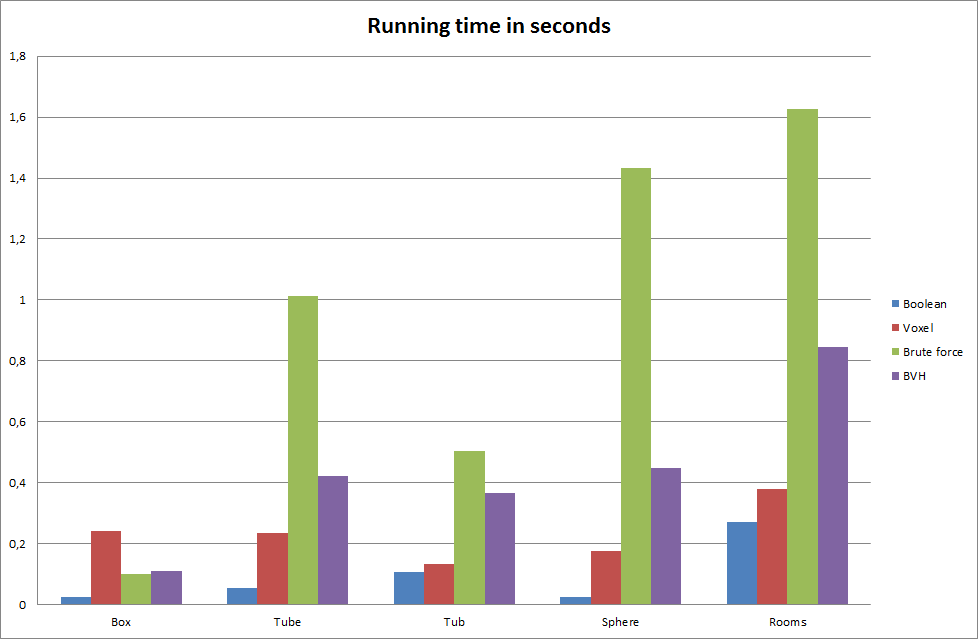
\includegraphics[width=0.45\linewidth]{images/running_time_seconds}
    \caption{Awesome Image}
    \label{fig:awesome_image1}
\end{figure}
\begin{figure}[h]
    \centering
    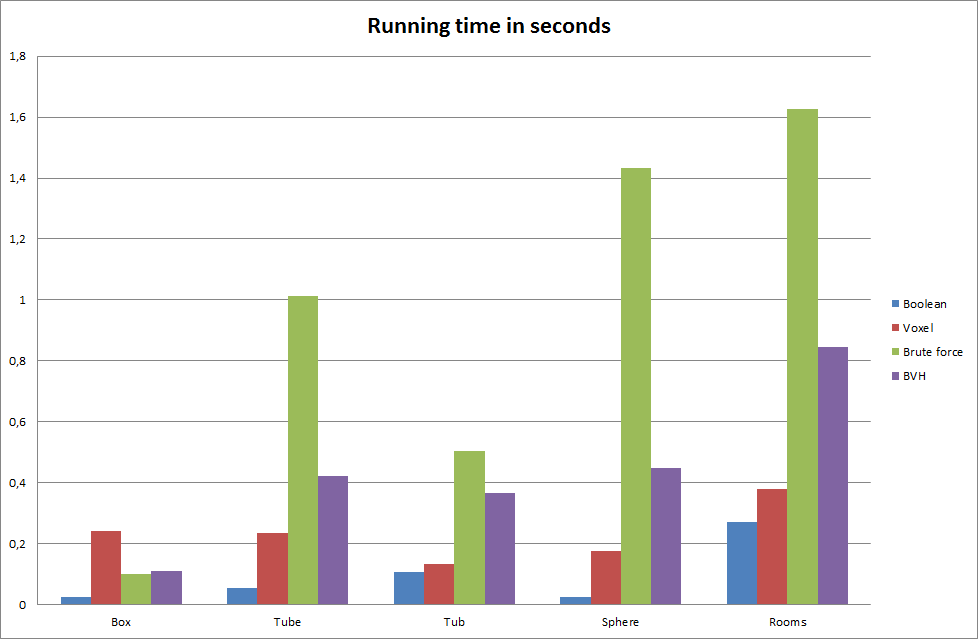
\includegraphics[width=0.45\textwidth]{images/running_time_seconds}
    \caption{Awesome Image}
    \label{fig:awesome_image2}
\end{figure}

This chapter will show the results. Figure~\ref{fig:awesome_image1} shows a photograph of a gull.

This \cite{wiki:123} cites wikipedia
\chapter{Discussion}

\chapter{Future Research and Conclusion}
This \cite{amanatides1987fast} sites something

\bibliographystyle{plain}
\bibliography{master}

\listoffigures
\listoftables
\appendix
\chapter{This is an appindex}
\section{First Appendix}
Hello world

\end{document}